\documentclass[border=5pt]{standalone}
\usepackage[utf8]{inputenc}
\usepackage{amssymb}
\usepackage{amsmath}
\usepackage{tikz}
\usetikzlibrary{arrows.meta}

\begin{document}
\nopagecolor
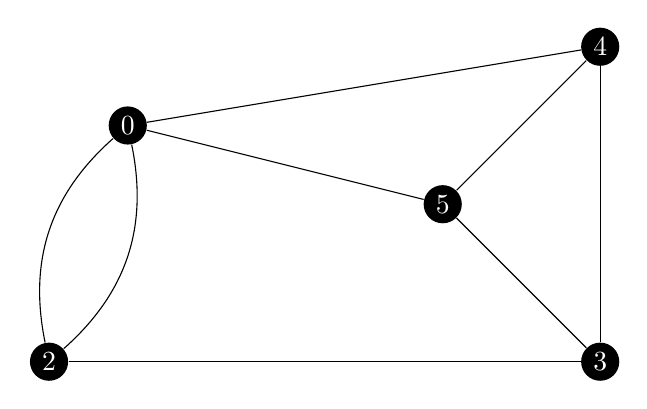
\begin{tikzpicture}
    \node[circle, inner sep=2pt, fill] (0) at (-2.5, 1) {\color{white} 0};
    \node[circle, inner sep=2pt, fill] (2) at (-3.5, -2) {\color{white} 2};
    \node[circle, inner sep=2pt, fill] (3) at (3.5, -2) {\color{white} 3};
    \node[circle, inner sep=2pt, fill] (4) at (3.5, 2) {\color{white} 4};
    \node[circle, inner sep=2pt, fill] (5) at (1.5, 0) {\color{white} 5};
    
    \draw (0) edge[bend right] (2)
          (0) edge (5)
          (0) edge[bend left] (2)
          (0) edge (4)
          (2) edge (3)
          (3) edge (4)
          (3) edge (5)
          (4) edge (5)
          ;
\end{tikzpicture}
\end{document}